% ============================================================
% SECTION: Data & QSAR
% ============================================================
\section{Data Ingestion \& QSAR Screening}

\begin{frame}{ChEMBL Bioactivity Layer}
  \begin{columns}[T]
    \begin{column}{0.55\textwidth}
      \begin{block}{ChEMBL Database}
        \begin{itemize}
          \item $>$19 million bioactivity records
          \item $>$2 million unique compounds
          \item Queried via REST API per target on demand
        \end{itemize}
      \end{block}
      \vspace{0.3cm}
      \begin{block}{Data Cleaning Pipeline}
        \begin{enumerate}
          \item Fetch IC50 (human assays, nM units)
          \item Validate SMILES via RDKit \texttt{MolFromSmiles}
          \item Deduplicate by Morgan fingerprint (catches tautomers \& stereoisomers)
          \item Drop grey zone: 1{,}000–10{,}000\,nM (ambiguous labels)
          \item Label: IC50 $\leq$ 1{,}000\,nM $\Rightarrow$ \textbf{active}
          \item Stratified 80/20 train/test split
        \end{enumerate}
      \end{block}
    \end{column}
    \begin{column}{0.42\textwidth}
      \begin{exampleblock}{SQLite Cache}
        All API responses cached locally (7-day TTL).
        Re-runs for the same target return in milliseconds.
      \end{exampleblock}
      \vspace{0.3cm}
      \begin{alertblock}{Label Noise Reduction}
        Compounds with IC50 in the 1–10\,µM range are
        removed before training: they are neither clearly
        active nor clearly inactive and inflate decision-
        boundary ambiguity in the binary classifier.
      \end{alertblock}
    \end{column}
  \end{columns}
\end{frame}

\begin{frame}{QSAR Model Architecture}
  \begin{columns}[T]
    \begin{column}{0.52\textwidth}
      \begin{block}{Molecular Featurisation}
        \textbf{Morgan Fingerprints} (radius\,=\,2, 1024 bits)\\
        Circular substructure encoding, invariant to SMILES
        notation.

        \vspace{0.25cm}
        \textbf{Physicochemical Descriptors} (6 features):
        \begin{itemize}
          \item Mol.\ weight, LogP
          \item H-bond donors (HBD), H-bond acceptors (HBA)
          \item Rotatable bonds, aromatic ring count
        \end{itemize}

        \vspace{0.2cm}
        Feature vector: $\mathbf{x} \in \mathbb{R}^{1030}$
      \end{block}
    \end{column}
    \begin{column}{0.45\textwidth}
      \begin{block}{Random Forest Classifier}
        \begin{itemize}
          \item 200 trees, \texttt{random\_state=42}
          \item 5-fold stratified cross-validation
          \item Metrics: CV ROC-AUC and held-out F1
          \item Serialised to \texttt{\{target\_id\}.pkl} after training
        \end{itemize}
      \end{block}
      \vspace{0.25cm}
      \begin{alertblock}{Why Classification?}
        Cross-assay IC50 noise degrades regression more than
        classification. \texttt{predict\_proba} already
        provides a continuous ranking signal.
      \end{alertblock}
    \end{column}
  \end{columns}
\end{frame}

\begin{frame}{QSAR Screening Results}
  \begin{center}
    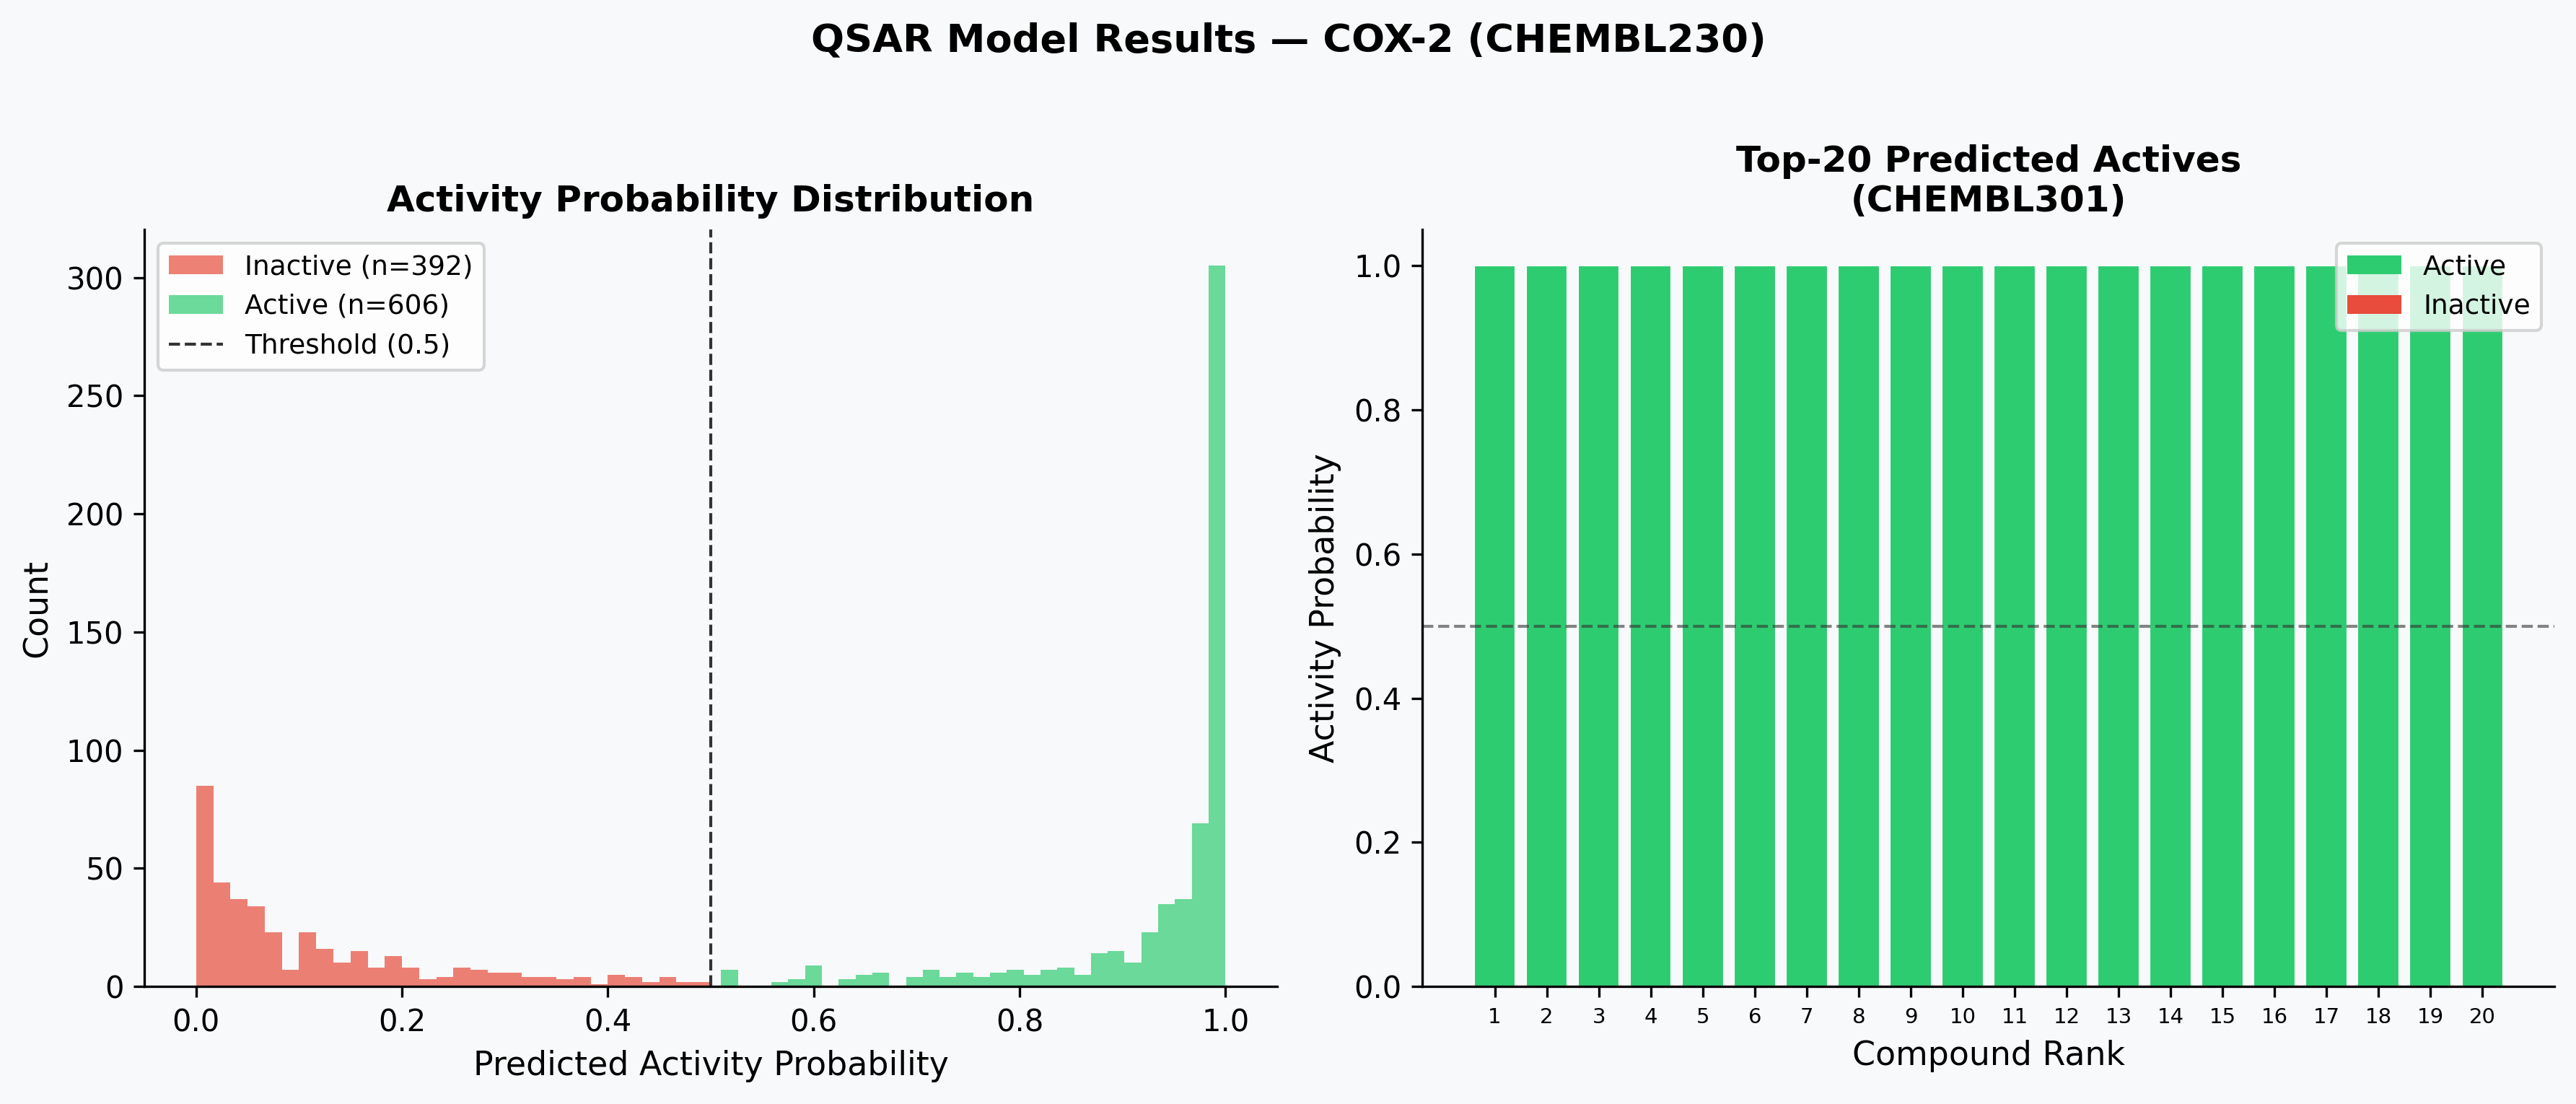
\includegraphics[width=0.88\textwidth]{../figs/qsar_metrics.png}
  \end{center}
  \textit{Left}: predicted activity probability distributions by true label.
  \textit{Right}: top-20 ranked compounds coloured by ground-truth activity.
  CDK2 (CHEMBL301) — CV AUC\,=\,0.943, Test F1\,=\,0.901, $n_\text{train}$\,=\,798.
\end{frame}

\begin{frame}{Candidate Pre-selection: Drug-likeness \& Diversity}
  \begin{columns}[T]
    \begin{column}{0.50\textwidth}
      \begin{block}{Step 1 — Lipinski Rule of Five}
        Drug-likeness gate applied to predicted actives:
        \begin{itemize}
          \item MW $\leq$ 500\,Da
          \item LogP $\leq$ 5
          \item HBD $\leq$ 5
          \item HBA $\leq$ 10
          \item TPSA $\leq$ 140\,\AA$^2$
        \end{itemize}
        \small Falls back to all actives if none pass.
      \end{block}
    \end{column}
    \begin{column}{0.47\textwidth}
      \begin{block}{Step 2 — Max-Min Diversity Selection}
        Greedy farthest-point algorithm on Tanimoto distance
        over Morgan fingerprints:
        \begin{enumerate}
          \item Seed: highest-$p$ drug-like compound
          \item Each step: add compound maximally distant
                from all already selected
          \item Stop at $N = 20$
        \end{enumerate}
        \vspace{0.1cm}
        \small $d_T(A,B) = 1 - \dfrac{|A \cap B|}{|A \cup B|}$
      \end{block}
    \end{column}
  \end{columns}
  \vspace{0.15cm}
  \begin{exampleblock}{Why Diversity?}
    Similar scaffolds share binding modes — a top-20 of structurally
    identical compounds wastes docking budget on a single binding hypothesis.
    Max-min selection maximises binding-pocket exploration.
  \end{exampleblock}
\end{frame}
